\chapter{Theory}
This is theory.
Have you seen my latest boat?
Kontiki-V!

\section{Cryptographic Hashing}

A cryptographic hash function, also commonly referred to as a digital signature or
a message digest, is a function that takes input data of varying size and
produces an output value of a constant size\cite{hashing-overview}. % That article is a pain to read

Cryptographic hash functions are designed to be one-way, meaning it should
be computationally not feasible to find the input data given the hash value,
and collision resistant, meaning that it should not be practical to find two
different sets of input data that produce the same output hash\cite{sha-spec}.

\section{The SHA-2 Algorithms}

The set of algorithms referred to as the SHA-2 algorithms are currently described in \cite{fips180-4},
and consists of algorithms for producing hashes with lengths of 224, 256, 384 and 512 bits.
The algorithms uses simple operations, limited to shifts, rotates, xor, and unsigned additions,
in addition to a lookup-table of constants, which allow for high-speed implementations in both
software and hardware. The different algorithms differ in how and with what parameters the various
operations are invoked.

\subsection{The SHA-256 Algorithm\cite{sha-spec}}

SHA-256 is the algorithm used in cryptocoin mining. It operates on blocks of 512 bits
and keeps a 256-bit intermediate hash value as state.

Before the first block is processed, the initial hash value is set to a predefined
value. The entire message that is to be hashed is then padded in what the standard
refers to as ``the usual way'', appending a 1 bit to the end of the message and then
appending zeroes until the length of the final block is 448 bits. Then the length of
the entire message, without padding, is added as a 64-bit integer to the end of the
block.

Then, each input block is split into 64 32-bit long expanded message blocks, $W_j$,
according to the formula

\[ W_j = \left\{
	\begin{array}{l l}
		M_j & \quad j \in \left[0, 15\right]\\
		\sigma_1(W_{j - 2}) + W_{j - 7} + \sigma_0(W-{j - 15}) + W_{j - 15} & \quad j \in \left[16, 63\right]
	\end{array}
\right.\]

\noindent where $M_j$ is the current input message block and the functions $\sigma_0$ and $\sigma_1$
are defined as

\[\sigma_0 = R^7(x) \oplus R^{18}(x) \oplus S^3(x)\]
\[\sigma_1 = R^{17}(x) \oplus R^{19}(x) \oplus S^{10}(x)\]

\noindent where the operator $R^n$ means right rotation by $n$ bits and $S^n$ means right shift by $n$
bits \footnote{Curiously, \cite{sha-spec} defines the operator $R$ to mean shift and $S$ to mean rotate.
We use the more intuitive definitions.}.

\subsubsection{The Compression Function}
The compression function is the core of the SHA-256 algorithm. It uses a lookup table
of 64 constants, $K_j$, and the following functions when calculating the new intermediate
hash values $a - h$:

\[Ch(x,y,z) = (x \wedge y) \oplus (\neg x \wedge z)\]
\[Maj(x, y, z) = (x \wedge y) \oplus (x \wedge z) \oplus (y \wedge z)\]
\[\Sigma_0(x) = R^2(x) \oplus R^{13}(x) \oplus R^{22}(x)\]
\[\Sigma_1(x) = R^6(x) \oplus R^{11}(x) \oplus R^{25}(x)\]

At the beginning of each iteration of the compression function, two temporary
values are calculated:

\[T_1 = h + \Sigma_1(e) + Ch(e, f, g) + K_j + W_j\]
\[T_2 = \Sigma_0(a) + Maj(a, b, c)\]

The new hash values are then assigned as follows:

\[\begin{array}{l}
	h \leftarrow g \\
	g \leftarrow f \\
	f \leftarrow e \\
	e \leftarrow d + T_1\\
	d \leftarrow c \\
	c \leftarrow b \\
	b \leftarrow a \\
	a \leftarrow T_1 + T_2 \\
\end{array}\]

The compression function is run 64 times, once for each extended message block,
$W_j$. When the final input block has been processed, the final hash is composed
by concatenating the intermediate hash values.

\section{Bitcoin Mining}

\todo{Move Bitcoin chapter from introduction}

\section{Direct Memory Access (DMA)}

Torbjørn deals with this one

\subsubsection{Brief history of DMA}

%TODO Qualify the introduction history, of polling and interrupts. Get coverage by reference.
\todo{Qualify the introduction history, of polling and interrupts. Get coverage by reference.}
Originally, the processors polled the different devices for data transfer requests. Most of the times, the polls returned negative answers, and this was concidered inefficient. An alternative to polling is interrupt requests, where the processor recieves an interrupt from a device requesting data transfer to or from the memory. This is more efficient than polling, since the processor does not have to keep polling the devices for requests. In both cases, however, the processor executes the data transfer.

Direct Memory Access (DMA) was developed in 19XX to leverage the processor from doing this type of data transfer between external devices. Typically use is that as soon as a processor receives a request from a peripheral device, it activates the DMA module. The DMA module receives the load address, the store address and a count of data to be transfered. While the DMA executes the data transfer, the CPU will work with other tasks, until the DMA module signalizes that it's done.

\subsubsection{Current network system in SHMAC}
\todo{Add reference to the SHMAC introduction paper, including pagenumber?}
%TODO Add reference to the SHMAC introduction paper, including pagenumber?
SHMAC implements a 2D mesh-based Network-on-a-Chip (NoC) interconnection network. 
Currently, the system uses dimension-ordered (XY) routing, and store-and forward switching with on/off flow control. 
The switching routine can be replaced in the future, should the current routine be found to cause performance bottelnecks.

\todo{Make sure the "goal"-part is valid}
%TODO Make sure the "goal"-part is valid
SHMAC does not implement DMA today, and data transfers are performed by the on-tile processors. 
A goal of this project is to explore the different options of implementing a DMA-module in the system, and create a test prototype that may be implemented in SHMAC.

\subsection{DMA module functionality}
\todo{Documentation, documentation, documentation!}
%TODO Documentation, documentation, documentation!
The minimum reguirement of a DMA-module is to transfer data from one location to another, while the CPUs of the system only have to send requests and receive interrupt signals.
The CPUs themselves should work on other tasks while the DMA-module transfers the data.
This is the minimum requirement, but for an efficient implementation for a given system, there are several options to consider.
\todo{"Given environment" sounds weird, must find better expression} 
%TODO "Given environment" sounds weird, must find better expression
Among these options are operation modes, transfer types, integration with the system, choice of registers and interruptions.
Architectural implementation of the DMA-module are affected by the chosen options, and how well they correspond with the SHMAC system.
The following subchapters will discuss these different options. 

\subsubsection{Operation modes}
\todo{WARNING: Got only Wikipedia on this. Document!}
%TODO WARNING: Got only Wikipedia on this. Document!
\textbf{WARNING: Got only Wikipedia on this. Document!}
Operation mode concerns about how the DMA operates on the network, in correspondance with other peripherals that also may need the use of the network.
There are three modes that are well known for shared media networks:
\begin{itemize}
    \item \textbf{Burst mode}.
    The DMA module has full ownership of the bus as long as the transfer is under execution.
    This is the fastest transfer operation for the DMA module, but it reduces the access for the CPU and other peripherals as long as the DMA is executing the transfer.
    In a shared network, the access will be blocked.
    \item \textbf{Cycle stealing mode}.
    The DMA requests the bus as in burst mode, but relents the control of the bus after transfering one byte of data.
    It will then re-request access to the bus for each transmission.
    In this way, the CPU and other peripherals may get needed access to the bus earlier compared to burst mode. 
    \item \textbf{Transparent mode}.
    DMA transfers data only when CPU is not performing operations that require access to the bus.
    This is the slowest operation mode for the DMA to finish, but also the one with best overall system performance, since the DMA has as few blocks as possible for the CPU. 
\end{itemize}
On a shared media network such as the one used on SHMAC, these implementations will be different.
But the principle remains the same: How much priority should a DMA transfer have, compared to other transfers on the system?
A fastest as possible transfer, like the burst mode, will make DMA transfer more efficient, but it will also add most the restriction on the network for other modules and peripherals, should it occur at a time when many peripherals/tiles performs data transfer.
A lower priority scheme will make these transfers go faster for other modules, but at the same time, DMA transfers will be slower.
\todo{This is outrageously based on an assumption, that priority schemes already exists. An assumption does not hold. Get this confirmed!}
%TODO This is outrageously based on an assumption, that priority schemes already exists. An assumption does not hold. Get this confirmed!
Deciding the priority of a DMA transfer, however, will be up to the routers in the network, and is therefore outside the scope of this current project.

\subsubsection{Transfer types}
\todo{These functions are from the manual of the PIC24F family by Microchip Inc. Add reference!}
%TODO These functions are from the manual of the PIC24F family by Microchip Inc. Add reference!
Transfer types describes how the load destination and the store destination are addressed.
They are both given a load and store address, but whether they change with an offset for each data transfer depends on the tranfer type.
INSERT REFERENCE HERE describes the following options:
\begin{itemize}
    \item \textbf{Fixed-to-fixed transfer}.
    Both load and store destination remain the same for each data transfer.
    \todo{Double check}
    This mode is suitable for transfers of single data between two fixed addresses, or if the DMA operates with signle transfers.
    \item \textbf{Fixed-to-block transfer}.
    The load address is fixed, while the store address increments.
    This is useful for storing data from a buffer of a serial communication peripheral.
    \todo{Find confirmation for this}
    It could also be used to do multiple copy of a data from a single address to multiple addresses.
    \item \textbf{Block-to-block transfer}.
    Both load and store addresses increments for each transfer.
    This is the scheme where entire blocks of data is transfered during a single operation.
    \todo{Perhaps mention this as a requirement?}
     \item \textbf{Block-to-fixed transfer}.
    Load address increments, while store address remains the same.
    This is useful when tranfering data into a buffer of a serial communications peripheral.
\end{itemize}

\subsubsection{System and data registers}
A DMA requires minimum a buffer for storing transfering data, as well as registers for load addresses and store addresses.
Counters and a register for maximum count is also needed when transfering blocks of data.
\todo{What is a channel?}
DMA modules often operates with multiple channels, each handling their own data transfers.
A possible implementation for multiple channels is to have seperate registers for load addresses, store addresses and counts for each channel.
Another possible implementation is to have a buffer for outgoing data, where request ID, load address and store address are combined in order to recognize the incomming data from the load memory and send them to the correct store address.
In this case, one counter may operate with one load address and generate the requests at the time.

\subsubsection{Tile vs. Accelerator on SHMAC}
\todo{Add a figure of each option}
\todo{Documentation, documentation, documentation... uhm... how do you document your separate ideas for the options?}

A DMA module may be implemented as a separate tile in SHMAC, as seen in figure \todo{Add figure} ADD FIGURE, or as an accelerator on an exisiting tile architecture, for instance the a CPU tile, as seen in figure \todo{Add figure} ADD FIGURE.
\\ There are different reasons for and agaist each option:
\begin{itemize}
    \item A full tile gives the benefit of having a full tile for the DMA implemenation allow.
    This is useful for complex implementations that require much space.
    However, for a simple implementation, a full tile may be a waste of space.
    \item As an accelerator, DMA may be implemented on already existing tiles.
    A tile may have parts of it powered down, therefore a DMA module may very well be implemented without any cost of power usage of the rest of the tile.
    In fact, a DMA module may work as only active part of a tile as well.
    A tile with a DMA module does not have to send out the request to an external tile either.
    But implementing on an existing tile architecture means sharing an internal shared bus network, and also less space for complex implemenations.
\end{itemize}
Which choice is the best, depends heavily on how DMA will be implemented on SHMAC, as the following sub-section will describe.

\subsubsection{Integration on SHMAC}
For a basic implementation of DMA, all that is needed for the DMA module to work is that it transfers from one address to another, when requested.
It does not need to know where in the system it is, and what route the data must take from the load address to the store address through itself.
Figure \ref{fig:DMASHMAC1} shows an excampe where DMA is implemented as a seperate tile, and works with the basic conditions.

\todo{Figure needs update, remove some texts and rename PU to CPU}
\begin{figure}[h!]
    \centering
%    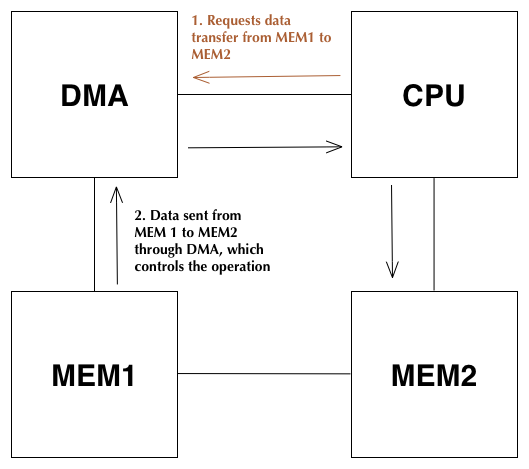
\includegraphics[width=0.7\textwidth]{Figures/DMA/DMASHMAC1}
    \caption{DMA module implemented as tile on SHMAC, with basic transfer from MEM1 to MEM2 through itself}
    \label{fig:DMASHMAC1}
\end{figure}
 
As it can be seen in the figure, the DMA tile recieves a request from its neighbour CPU tile, and performs loads and stores from the tile MEM1 to the tile MEM2.
This would also work the same way if the DMA-module was implemented on the CPU tile as an accelerator instead.
While this completes the basic goal of moving data on behalf of the CPU tile, it does not know or care where in the SHMAC system it is.
If two memory tiles are close to each other, while the active DMA tile is far away (for instance on the other side of the entire SHMAC board), the data would have to travel unnecessary far to reach the goal, and the entire operation will slow down.
Figure \ref{fig:DMASHMAC2} shows an implementation where the DMA tile lures MEM1 to believe that MEM2 requests the data, and loads out the data, while MEM2 stores the recieved data.
This could be done by sending a request signal through MEM2 to MEM1 with packet info claiming that the requestor is MEM2. 

\begin{figure}[h!]
    \centering
%    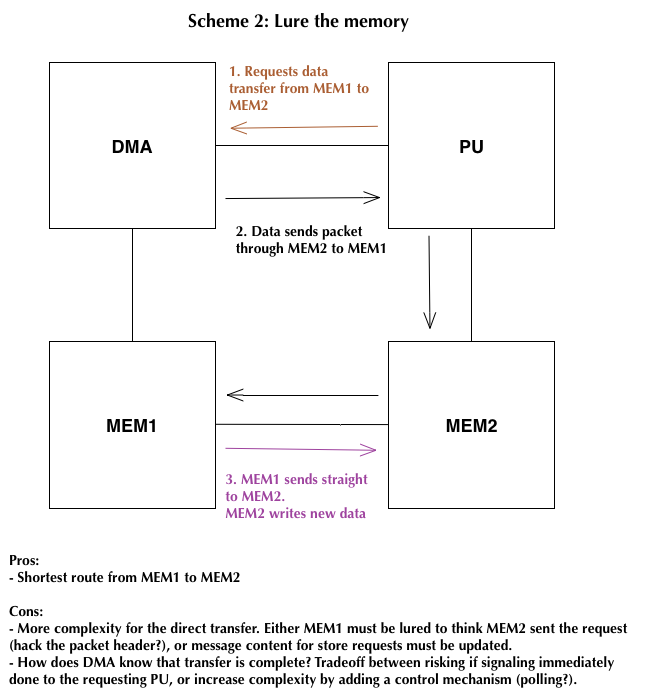
\includegraphics[width=0.7\textwidth]{Figures/DMA/DMASHMAC2}
    \caption{DMA implemented with luring MEM1 to load data to MEM2}
    \label{fig:DMASHMAC2}
\end{figure}
 
This way, the distance is as short as possible, but how does the DMA tile know when the transfer is done, since it is not doing the tranfer itself?
It could ignore this task and signal the CPU that the transfer is complete as soon as the luring request has been sent out, but depending on the storing tile (a memory tile, or another accelerator tile), the CPU will risk loading old data that has not yet been overwritten, should it load from the "wrong" address too early, before new data has arrived.
Alternatively, the DMA module may be implemented with polling, so that it polls the MEM2 tile to see the data transfer is complete.
This does lead to futher complexety in implementing the DMA.
How does it know when new data transfer is complete?
 
\begin{figure}[h!]
    \centering
%    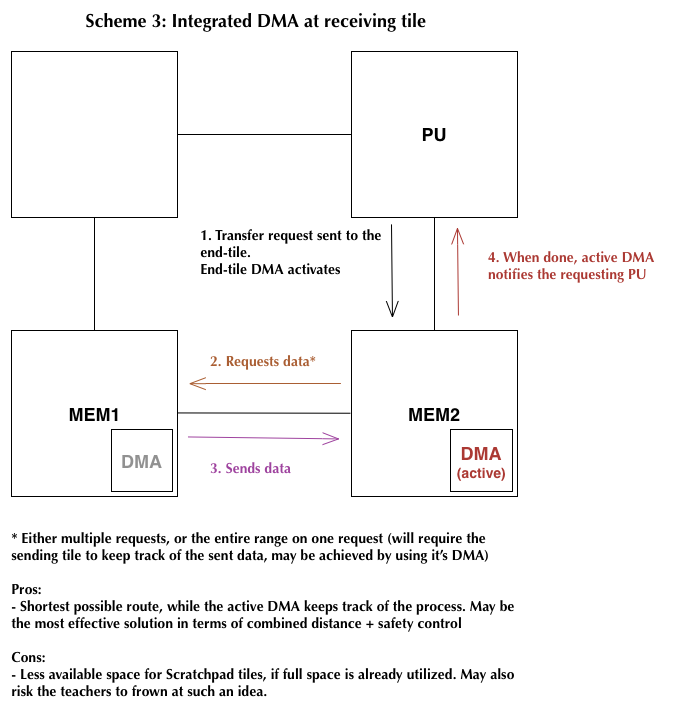
\includegraphics[width=0.7\textwidth]{Figures/DMA/DMASHMAC3}
    \caption{DMA module implemented directly on storing memory tile}
    \label{fig:DMASHMAC3}
\end{figure}
 
Figure \ref{fig:DMASHMAC3} shows an implementation where the DMA module has been implemented on the memory tiles themselves.
In this scheme, the CPU sends the DMA transfer request to the DMA on the storing tile.
As soon as the request reaches the DMA module on MEM2, it will generate load requests to MEM1.
As soon as data arrives, the DMA module will store the data in the store addresses, and signal the requesting CPU when the task is done.
In this example, the distance between MEM1 and MEM2 is as short as possible, anwd the DMA module keeps the transfer safe since it knows when the task is complete before signaling the CPU.
The main drawback, however, is that by implementing the DMA module directly on the memory tile, there will be less space for memory itself.
The DMA module or the entire operation will also be more complex, for the following reasons:
Either the DMA module itself must know where it is in the system, before either passing on the request to the correct DMA Module on the correct tile, or the requesting CPU itself must know where the correct DMA module is (either by checking a look-up table, or deducing based on the location of the storing data address).
In the first case, the DMA module must be implemented with knowledge of its own position, and with the ability to pass on requests to the correct module.
This itself increases the complexity of the module. \todo{But also add favorable reasons?} 
Finally, another question arises: Whould the DMA Module in MEM2 send multiple single load requests to MEM1, or should it cooperate with the DMA module on MEM1 by sending only the start address and the load offset, and letting the module on MEM1 load and send out the data?
The latter case would be more efficient in terms of data transport, as only one request from MEM2 to MEM1 would be necessary, but at the same time implementing a cooperation scheme between two DMA modules would futher increase the complexity of the implementation.
On a memory tile, futher complexity also means less memory space.
In summary, this is a compromizing choice between memory size, and efficiency.
 
\subsubsection{Cache coherency issues}
In SHMAC, data that is shared among more than one processing units, are currently found only on uncachable memory area.
What do we do with multiple DMA writes to same uncachable area?
TBA.

\subsubsection{Issues with virtual memory}
Currently, SHMAC does not implement virtual memory, but since it is planned to implement, it has to be addressed as well.
It's nothing personal, Jack. It's just good business. 


\subsubsection{Other options to consider}
What is the data size? 
Byte or bit? 
Who can interrupt? 
What type of interruptions may the DMA send out? 
Multiple jobs?
Generic DMA or specialized DMAs?


\subsection{Chosen solution}

Description of chosen DMA-description, and why.
Maybe mention alternatives/recommendations that may be picked up should things go wrong.
\\
Section may also be moved to methology

\subsubsection{Assumptions for the project}
All data are transfered sequential, due to the XY routing that is implemented.
Data does not arrive out of order.


















